\begin{figure}[t]
\begin{center}
\begin{small}
\begin{sc}
\begin{center}
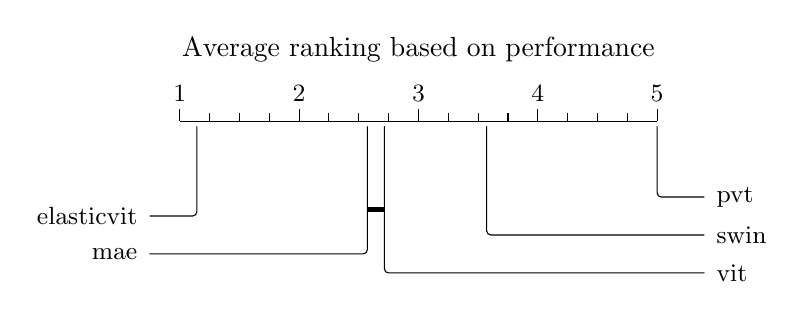
\begin{tikzpicture}[
  treatment line/.style={rounded corners=1.5pt, line cap=round, shorten >=1pt},
  treatment label/.style={font=\small},
  group line/.style={ultra thick},
]

\begin{axis}[
  clip={false},
  axis x line={center},
  axis y line={none},
  axis line style={-},
  xmin={1},
  ymax={0},
  scale only axis={true},
  width={.5\linewidth},
  ticklabel style={anchor=south, yshift=1.3*\pgfkeysvalueof{/pgfplots/major tick length}, font=\small},
  every tick/.style={draw=black},
  major tick style={yshift=.5*\pgfkeysvalueof{/pgfplots/major tick length}},
  minor tick style={yshift=.5*\pgfkeysvalueof{/pgfplots/minor tick length}},
  title style={yshift=\baselineskip},
  xmax={5},
  ymin={-3.5},
  height={4\baselineskip},
  xtick={1,2,3,4,5},
  minor x tick num={3},
  title={Average ranking based on performance},
]

\draw[treatment line] ([yshift=-2pt] axis cs:1.1428571428571428, 0) |- (axis cs:0.726190476190476, -2.5)
  node[treatment label, anchor=east] {elasticvit};
\draw[treatment line] ([yshift=-2pt] axis cs:2.5714285714285716, 0) |- (axis cs:0.726190476190476, -3.5)
  node[treatment label, anchor=east] {mae};
\draw[treatment line] ([yshift=-2pt] axis cs:2.7142857142857144, 0) |- (axis cs:5.416666666666667, -4.0)
  node[treatment label, anchor=west] {vit};
\draw[treatment line] ([yshift=-2pt] axis cs:3.5714285714285716, 0) |- (axis cs:5.416666666666667, -3.0)
  node[treatment label, anchor=west] {swin};
\draw[treatment line] ([yshift=-2pt] axis cs:5.0, 0) |- (axis cs:5.416666666666667, -2.0)
  node[treatment label, anchor=west] {pvt};
\draw[group line] (axis cs:2.5714285714285716, -2.3333333333333335) -- (axis cs:2.7142857142857144, -2.3333333333333335);

\end{axis}
\end{tikzpicture}
\end{center}
\end{sc}
\end{small}
\end{center}
\afterplot
\caption{\textbf{Critical difference diagram}: Average performance ranking of \ours{} and baseline methods for ImageNet with high perturbation (most extreme settings). \ours{} significantly outperforms remaining approaches, while more structured methods (PVT and Swin) perform significantly worse than simple ViT. Moreover, the difference between ViT and MAE is insignificant. Notice that this diagram was generated for rankings generated based on results from Fig.~4 and Fig.~5 of the main paper. %~\ref{fig:zoom-sample}, \ref{fig:dropout-sample}, \ref{fig:shake-sample}, and \ref{fig:mixes}.
}
\label{fig:critdist}
\end{figure}